\begin{figure}[tbp]
\scriptsize
\begin{tabular}{p{4.5cm}p{2cm}}
%VisualGenome+ManyNames & \cite{snodgrass}\\
\centering
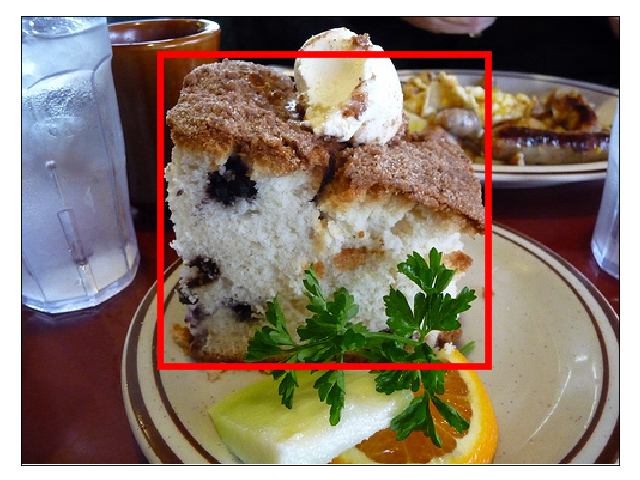
\includegraphics[scale=0.15]{figures/2390077_1254219_supercat_unique.png} &
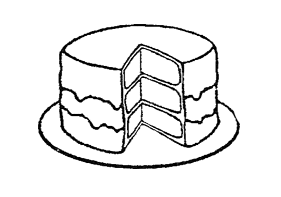
\includegraphics[scale=0.4]{figures/snodgrass_vanderwart_cake_042.png}\\
 cake (53),  food (19), bread (8), burger (6), dessert (6), snacks (3), muffin (3),  pastry (3) & \hspace{0.5cm} cake (83)
\end{tabular}
\caption{Names for a cake object in ManyNames (left) and in \citet{snodgrass} (right), percentages of responses in parentheses.}
\label{fig:cake}
\vspace{-0.5cm}
\end{figure}

Generally, research in Language \& Vision (L\&V) is interested in modeling how speakers \textit{naturally} name, refer to or talk about visual objects and scenes, in contrast to predicting abstract object labels as e.g.\ in Computer Vision.
This typically entails that data collections and models need to account for linguistic variation, as there can hardly ever be a single ground-truth utterance when referring to some visual entity. 
While variation has indeed been accounted for in many L\&V tasks, cf.\ work on image captioning \cite{Bernardietal:automatic}, object naming has been addressed in a comparatively simplistic way: 
even corpora with massive annotation like VisualGenome~\cite[\vg henceforth]{krishna2016visualgenome} typically provide a single label for each object assumed to be its canonical category or name.

%While many of these tasks are well-known to 
%\gbt{I've left only one image in the figure to highlight that we study variation for the same instance.}
%However, so far research in NLP has had surprisingly little to say about object naming.
%Neighboring areas
%, specifically Computer Vision and Cognitive Science, 
%have addressed related tasks, with simplifications that NLP is equipped to address:
%In Computer Vision, naming is usually equated with object categorization, and addressed as a classification problem in which a single label is provided for each object~\cite{googlenet}.
%In a typical evaluation, alternative names for the object in Figure \ref{fig:cake} such as \refexp{cake}, \refexp{dessert}, \refexp{sweet}, or \refexp{food} would be counted as incorrect.
%In Cognitive Science, object naming has received more attention, but it has been studied with stylized drawings instead of realistic images.
%, such that it is unclear how findings generalize to tasks in language \& vision.

We take a first step at studying natural naming of objects in real-world images and contribute a new dataset, ManyNames, that contains 36 crowd-sourced names for 25K instances from \vg.
Thus, our images show objects in complex visual contexts,
unlike the ``clean'' ImageNet data~\cite{imagenet_cvpr09} that has been previously used to train object classifiers \cite{ILSVRC15}, and unlike stylized line drawings used in picture naming experiments in Cognitive Science (see Figure \ref{fig:cake}).

As illustrated for an object of the class ``cake'' in Figure \ref{fig:cake}, our data reveals clear naming preferences (53\% of the annotators prefer the basic-level \textit{cake}) and also rich variation (the remaining annotators prefer other options like \textit{food, dessert, bread}) which is not restricted to taxonomical relations studied in previous work on naming \cite{rosch1976basic,Ordonez:2016,graf2016animal}. 
%We find both consistency and variation in naming: In instances, the relative frequency of the most common name is 75\% on average, which is remarkable for a task where subjects are allowed to produce whatever name they like. However, 
%there are still around 3 names being produced for each instance on average.
%Moreover, 
%we find a high level of variation within what would be considered a class in visual object recognition, with around 30 names per class.
%standard Computer Vision approaches (objects assigned the same synset in VisualGenome)
%Interestingly, most of this variation comes from alternative names that do not stand in a taxonomic relation, but range from 
%We also find a very high standard deviation in the agreement measures, which suggests that visual features (how prototypical the instance is of a given category, how clearly delimited the object is) are crucial factors determining variation.
%Our data also show that object identification via bounding boxes is not a trivial matter even for humans, with name variants ranging from clearly different objects in 
%cross-classifification  (\textit{cheesecake}-\textit{dessert}) to cases
% where it is visually impossible to distinguish between the two (\textit{bed}-\textit{bedsheet} when the bed is only partially shown) to cases 
%of near-metonymy (\textit{floor}-\textit{carpet}) and issues in object idenitification due to bounding boxes (\textit{man}-\textit{helmet}).
%Given these findings, we ask whether current models implicitly capture object naming variation of the sort provided by humans.
Interestingly, when testing a model of object recognition, that has been trained on \vg, on ManyNames, we observe better performance than on \vg.
%: It has 77\% accuracy when taking the most frequent ManyNames name as gold standard, vs.\ only 69\% on the VisualGenome name.
This suggests that object names annotated by many speakers provide a more robust ground for testing computational models, while also offering rich data for studying linguistic variation in naming.

% \item most of the variation in our dataset comes from alternative names that do not stand in a taxonomic relation, suggesting that the previous work in Cognitive Science is missing much of the empirical ground.
% %while previous work has mostly focused on variation in the level of generality within a taxonomy (\emph{penguin} vs. \emph{bird}), 

% our datasets contains a lot of variability for names coming from different parts of the taxonomy (\emph{dessert} vs. \emph{cake}, \emph{bottle} vs. \emph{wine})
% \end{itemize}

% Moreover, we analyze whether current models implicitly encode the variation in naming, by doing XXX. We find YYY.


% Our paper puts together two strands of research that have mostly been pursued independently to date.
% On the one hand, state-of-the-art computer vision systems are able to accurately classify images into thousands of different categories (e.g.\  \newcite{googlenet}), where the task is often to predict the class for a given object. 
%name for a given object. \gbt{Is this true? Imagenet task asks for synsets, which can be taken to be categories\dots To refine}
% However, they mostly adopt very simple assumptions with respect to the underlying lexicon, which is implemented by using single "ground truth" labels: 
%as a simple, flat labeling scheme:
 % A standard object recognition system would be trained to classify the left object in Figure~\ref{fig:cake} as \emph{cheesecake}, the right one as \emph{dessert}, and using \emph{dessert} for the left picture would be considered incorrect. 
% On the other hand, research on object naming in Cognitive Science has shown that people choose different names depending on the circumstances, with factors such as context or the prototypicality of the object with respect to the category playing a role~\cite{add-refs}. 
% \gbt{This research also argues that there is high agreement in how people name objects; to do: make coherent.}
% However, this research typically uses stylized drawings are used, and is focused on taxonomic relations (\textit{sparrow}-\textit{bird}).
% \sz{It is thus unclear how findings from these stylized settings generalize to tasks in language \& vision like referring expression generation, where naming is a core aspect. Therefore, in contrast to traditional naming norm studies in Cognitive Science we study object naming in realistic scenes where objects are situated in a natural context! (This comes with additional challenges, like potential object occlusion, background/foreground confusion etc.)}

% Seminal work on prototypes suggests that the prototypicality of the object will determine the level of generality of the object name, i.e.\  a robin can be named \emph{bird}, but a penguin is better referred to as ``\emph{penguin}'' \cite{Rosch1978}.

% Two main findings in the literature:

% \begin{itemize}
% \item very high agreement, most people use the same name for the same object
% \item prototypicality is a factor, context too, but research has only looked at generality/specificity of the name
% \end{itemize}

%The real-world objects that we interact with in our every-day life can be categorized into many thousands and maybe millions of categories. And even a single object can be member of many categories, i.e.\ at different taxonomical levels or in different parts of a taxonomy. For instance, both objects in Figure \ref{fig:cake} are at once instances of \cat{cake}, \cat{cheesecake}, \cat{dessert}, \cat{sweet}, \cat{pastry}, \cat{food} etc. Hence, when speakers name objects, e.g.\ when referring, they have to select a lexical item from a complex network of concepts and competing lexical alternatives.

%To date, research in NLP has surprisingly little to say about object naming, despite the fact that
% there has been a recent explosion of interest in various, and even complex, language \& vision tasks ranging from image captioning \cite{fangetal:2015,devlin:imcaqui,Bernardietal:automatic} to e.g.\ visual dialogue \cite{das2017visual,vries2017guesswhat}. 
%In contrast, closely related areas, such as computer vision and cognitive science, have investigated very related tasks in quite some depth: object recognition systems developed in the area of computer vision  are now able to classify images into thousands of different categories (e.g.\  \newcite{googlenet}).
%Furthermore, work on concepts, following the seminal work by Rosch, suggests that objects are typically conceptualized at a preferred level of specificity called the \textbf{entry-level}. Psycho-linguistic studies have been able to support this theory based on collections of so-called object naming norms. 
%
%This paper aims at addressing the genuinely linguistic questions revolving around the phenomenon of object naming by (i) presenting a collection of high-quality, large-scale naming data,  and (ii) analysis methods for this data and (iii) a first baseline model that accounts for the semantic flexibility of names for objects in real-world images. From computer vision, we borrow the idea of modeling realistic visual objects in realistic scenes (real-world images), but go beyond the simplistic assumption that object names correspond to unambiguous labels in a flat classification scheme (with no conceptual relations between the labels). From psycholinguistics, we borrow the idea of eliciting natural, representative naming data from many subjects, but go beyond using artificial, highly stylized objects.

%%% Local Variables:
%%% mode: latex
%%% TeX-master: "main"
%%% End:
